\chapter{Desenvolvimento do Jogo}\label{ch:Desenvolvimento}

%A documentação do jogo é o Game Design Document (ou GDD para os íntimos). Alguns chamam também de Game Design Bible. É a mesma coisa

O processo de desenvolvimento de jogos digitais é uma tarefa que exige do(s) desenvolvedor(es) conhecimentos de programação. Um jogo para ser desenvolvido, deve ser escrito em uma determinada linguagem de programação, o que acaba por obrigar que o(s) desenvolver(es) do jogo tenha(m) conhecimento sobre esta linguagem. Embora existam linguagens de programação visual, o conhecimento sobre lógica de programação ainda é parte fundamental para o desenvolvimento de um jogo. 

%(programação em blocos ou Visual Scripting) : linguagem de programação visual. 

Um jogo digital requer conhecimentos computacionais específicos para o seu desenvolvimento. Os jogos sérios, além de exigirem estes mesmo conhecimentos, devem ser desenvolvidos sobre príncipios pedagógicos e metodológicos de ensino. Sendo assim, a \autoref{sec:motor} descrever os principais aspectos computacionais levados em consideração para o desenvolvimento de um jogo sério voltado para prevenção da violência sexual infantil. Já a \autoref{sec:DN} discorre sobre a estrutura metodologica de ensino e a forma como esta se organiza sobre os níveis do jogo. É fundamental salientar aqui que, embora aspectos artísticos, sonoros, ergonomicos, estéticos e jurídicos sejam importantes no desenvolvimento de jogos, eles não são abordados neste trabalho, assim como questões sobre criptografia e banco de dados.




%Embora importantes no cenário de desenvolvimentos de jogos, aspectos artísticos, sonoros, ergonomicos, estéticos, aspectos jurídicos. 

%criptografia, banco de dados,

%demais aspectos de correspondem a infraestrutura não serão abordadaos. 


\section{Motor de Jogo}\label{sec:motor}

Motor de jogo (\textit{Game Engine}) é o nome dado a qualquer plataforma voltada para o desenvolvimento de jogos. Os motores de jogos proporcionam um ambiente completo para a criação de jogos, com toda a parte gráfica e sonoro já abstraídas. Isso permite ao desenvolvedor exportar o jogo para diferentes sistemas computacionais realizando alterações mínimas no código-fonte \cite{bishop1998designing, machado2009serious}. 

Existem vários motores voltados para o desenvolvilmento de jogos. O motor usado neste trabalho é o Godot\footnote{Godot é um motor de jogos totalmente gratuito e de código aberto sob a licença permissiva do MIT. O motor pode ser adquirido por meio do seguinte endereço: \url{https://godotengine.org/}} (versão 3.2). Em comparação aos demais motores de jogos, o Godot se destaca por ser totalmente gratuito, adaptado ao idioma português e por exportar os jogos para multiplos sistemas \cite{scherer2020analise}. Salienta-se que a última versão estável da plataforma Godot é a versão 3.2. Por tal razão essa é a versão que foi utilizada durante o andamento deste trabalho. Embora a plataforma exporte seus jogos para multiplos sistemas, é importante destacara que o jogo desenvolvido neste trabalho está exportado apenas para navegadores. %futuramente busca-se exportar o jogo para sistemas operacionais móveis, removendo assim a necessidade de conexão com a internet para se acessar o jogo. 
%Todo o processo de desenvolvimento do jogo ocorre em ambinete Linux, as linguagem utilizadas durante o processo de desenvolvimento são as liguagem ofertadas pelo Godot (C, C++), além de SQL e PHP para o gerenciamento e organização das informações em um banco de dados. 






%\section{Ensinamento}\label{sec:ensinamento}

%Os participantes devem ser capazes de identificar corretamente a localização e o nome das partes do corpo.

%As crianças devem saber diferenciar as partes íntimas do corpo das demais partes. 

%Os participantes devem manifestar competências sobre o uso seguro das tecnologias da informação e comunicação.

%As crianças devem saber reconhecer um adulto em quem possam confiar.

\section{Desenho de Níveis e Ensinamentos}\label{sec:DN}

O jogo para prevenção da violência sexual infantil projetado neste trabalho é do estilo aventura. Os jogos de aventura são jogos em que o jogador assume o papel de um protagonista em uma história interativa com exploração e resolução de quebra-cabeças. Os quebra-cabeças do presente jogo se traduzem em minijogos voltados a prevenção da violência sexual infantil. Ao se tratar do público infantil, observou-se que o estilo aventura, se destaca como o estilo de jogo que mais agrada de forma igualitária, meninos e meninas \cite{brandtzaeg2009children}. %tudo bem que são criança do norte da europa, maz fazer o que :P

\vspace{-0.1cm}

O jogo densenvolvido permite a customização de personagem. Esse recurso gera um elo entre personagem e jogador, porporcionam que o jogador possa se sentir representado no jogo. Além disso, o jogo possui um sistema de tutorial baseado em um personagem que acompanha o jogador. Esse sistema de ajuda ao jogador é implementado para facilitar o aprendizado sobre o jogo e suas dinâmicas \cite{buchinger2014sherlock}. Junto a este sistema de ajuda ao jogador, também é implementado a dinâmica herói mudo ou dinâmica do protagonista silencioso. 

\vspace{-0.1cm}

A dinâmica do herói mudo permite uma imersão maior ao jogador. Nessa dinâmica, o personagem do jogador não se expressa de maneira verbal \cite{domsch2017dialogue}. Graças a isso, não há o risco do personagem do jogador se utilizar de palavras ou de elementos contextuais que o jogador desconheça, proporciona assim, uma conexão maior entre personagem e jogador. Como artíficio, para dar enredo a história do jogo, as frases são transferidas para um personagem que o jogador não possui controle (o personagem tutor), com o intuito de evitar assim, uma disrupção da interligação entre personagem e jogador. Embora o personagem do jogador não fale; todos os diálogos do jogo são transcritos textualmente e verbalmente. A dublagem associada ao texto escrito proporciona acessabilidado do jogo as crianças que não encontram-se plenamente alfabetizadas \cite{limeira2015avaliaccao}. 

\vspace{-0.1cm}

%A prática de protagonistas silenciosos era utilizada no princípio do desenvolvimento de jogos devido a limitações tecnológicas, posteriormente se fez presente em histórias simples que não requeriam diálogo para narrar seus acontecimentos \cite{domsch2017dialogue}. Com a evolução da tecnologia, as empresas optaram em trazer um maior realismo aos jogos, no entanto a dinâmica do herói mudo permite uma imersão maior ao jogador, pois permite uma conexão maior entre personagem e jogador, uma vez que não há o risco do personagem se utilizar de palavras ou de elementos contextuais que o usuário desconheça. Nesse sentido, as perguntas são transferidas para um personagem que o jogador não possui controle (o personagem tutor), com o intuito de evitar assim, uma disrupção da interligação entre personagem e jogador.

Com o objetivo de abstrair e elucidar melhor alguns conceitos do jogo formulou-se o diagrama de atividades do jogo, representado na \autoref{fig:Diagrama}. Um diagrama de atividade é essencialmente um fluxograma que mostra as atividades executadas por um sistema. Tradicionalmente em diagramas, o início de um processo é representado por um círculo preenchido; o final de um processo é representado por um círculo preenchido dentro de outro círculo; os retângulos com cantos arredondados representam atividades que devem ser realizadas; as setas representam a passagem de uma atividade para outra; o losango representa uma decisão; o paralelogramo representa a inserção de informações; o cilindro representa o banco de dados; o retângulo esticado representa a junção de atividades; o retângulo com linhas internas representa o armazenamento interno; o semi-retângulo circular representa um tempo de espera; e o pseudo-triângulo invertido representa uma atividade externa a aplicação.





\begin{figure}[hbt!]
\caption{\label{fig:Diagrama}Diagrama de Atividades do Jogo}\vspace{-0.4cm}
\begin{center}
  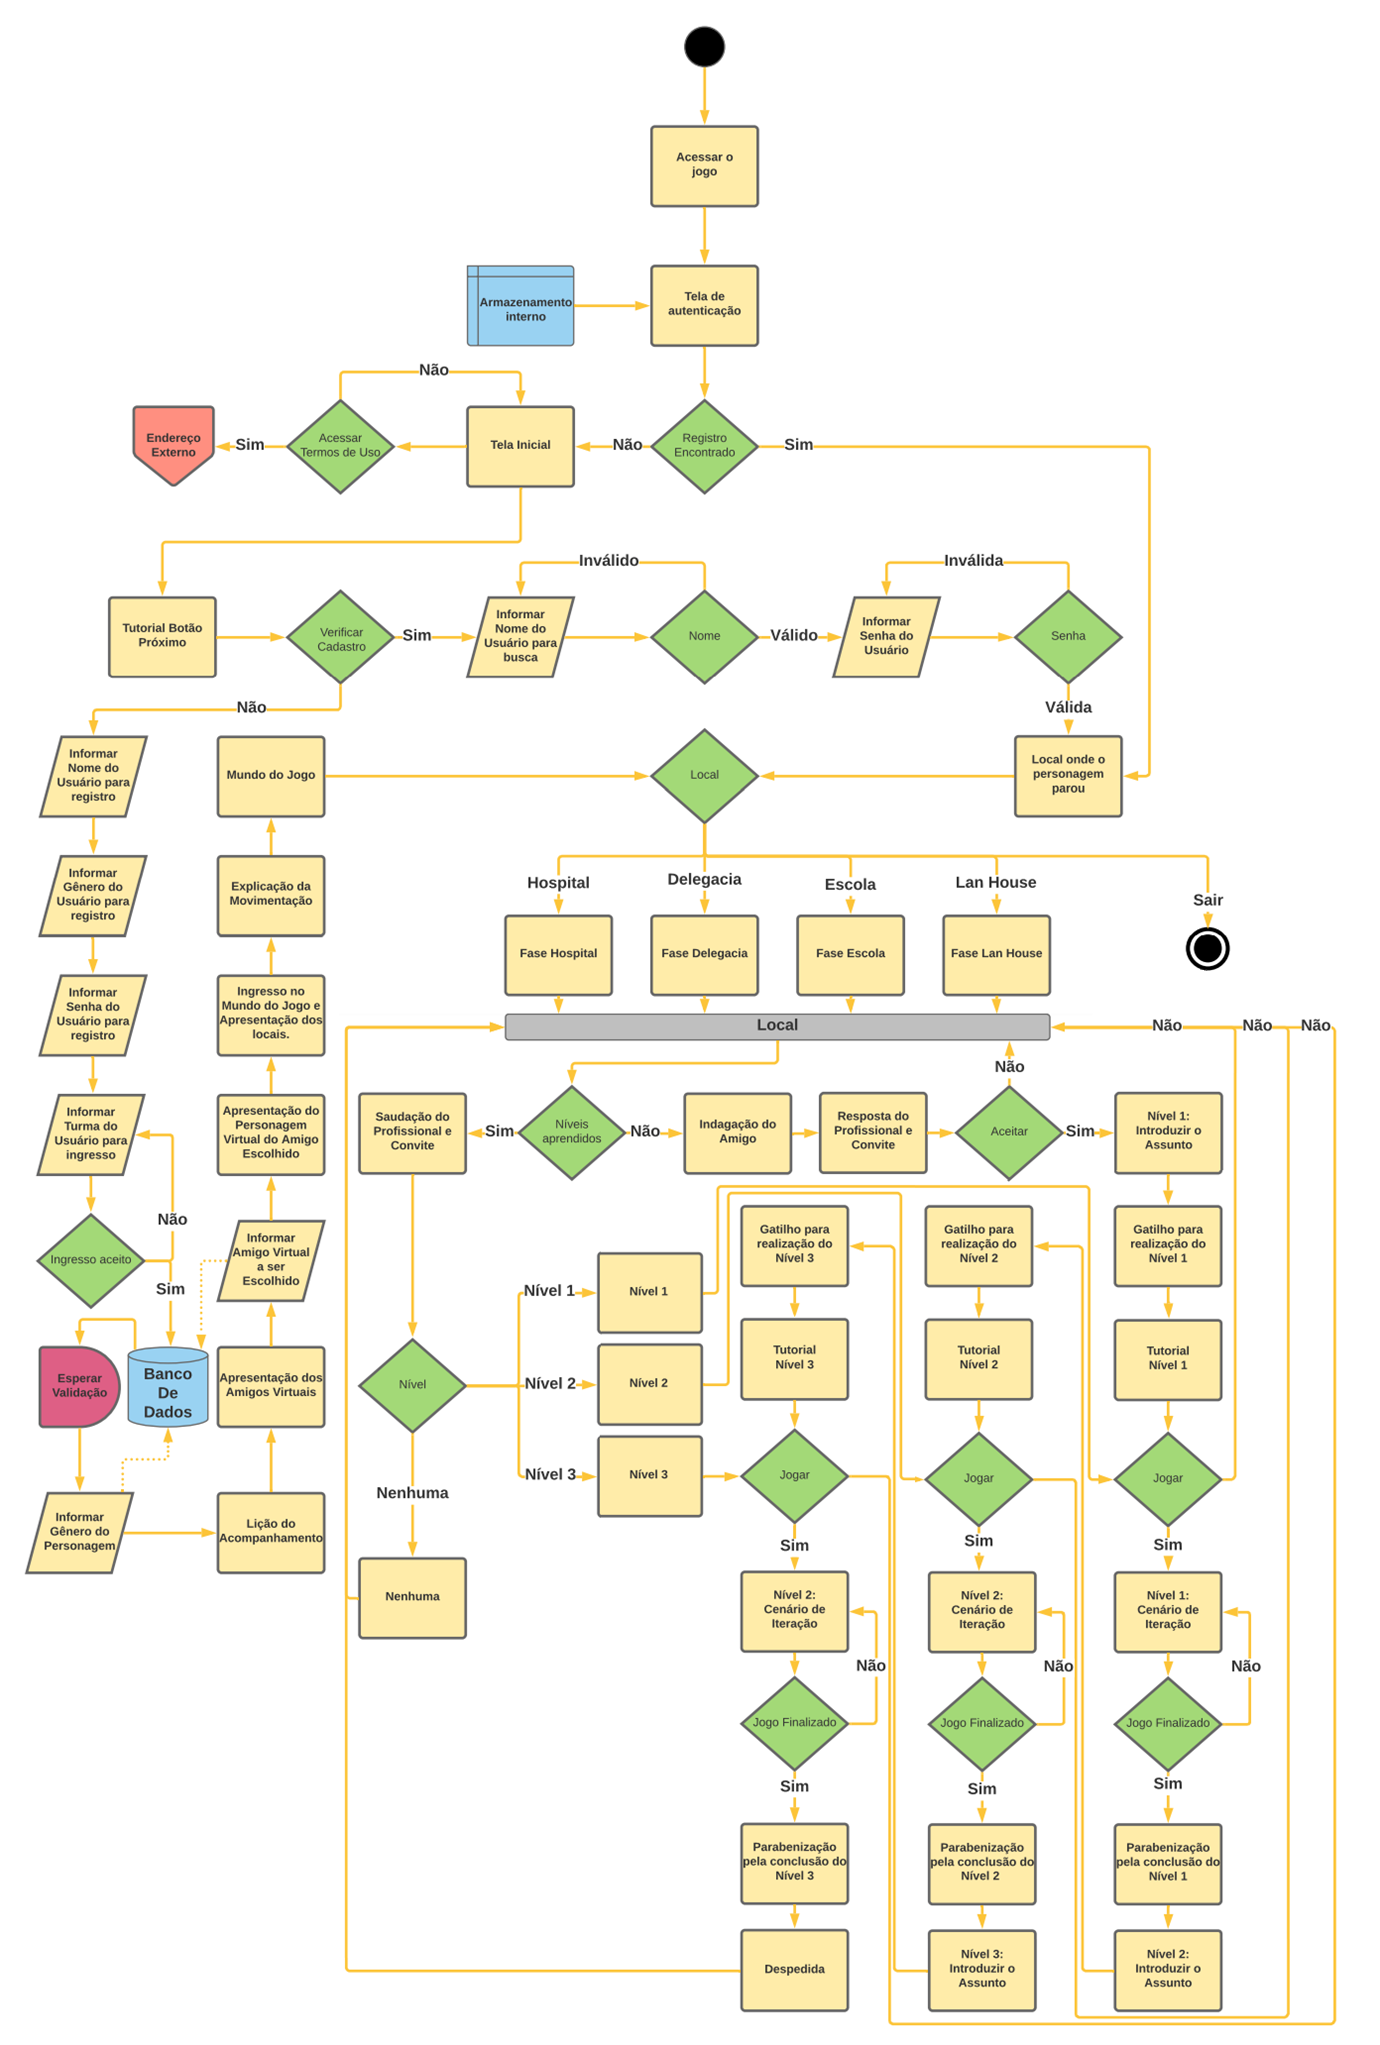
\includegraphics[width=0.95\linewidth]{./Figuras/DiagramaJoginho.png}
  \end{center}\vspace{-0.6cm}
\legend{Fonte: os autores}

\end{figure}


O diagrama de atividades da \autoref{fig:Diagrama}, representa de forma gráfica o fluxo de etapas necessárias para concluir cada atividade do jogo. A parte supeior corresponde as atividades relacionados ao acesso ao jogo. As atividades relacionadas ao cadastro no jogo é representados na parte esquerda do diagrama. Todas as demais atividades representadas no diagramas correspondem ao jogo em si. São quatro fases presentes no jogo: Fase do Hospital, Fase da Delegacia, Fase da Escola e Fase da Lan House. Cada fase possui três nível, em cada nível os jogadores aprendem conteúdos relacionados a prevenção da violência sexual infantil. 




Primeira fase..

Segunda fase..

Terceira fase..

Quarta fase..



\begin{comment}
propósito

Orientações em Sexualidade

Plataforma

Publico Alvo

Estilo

Estética

Arte

Fonte

Escalabilidade/Flexibilidade

Audio

Musica

Leiaute de Níveis

UX

Gamificação

Ergonomia de Botões

Artefato

Licença

Termos de Serviço

Política de Privacidade

Criptografia

Banco de Dados
\end{comment}

%%%%%%%%%%O enredo é tão importante para jogos sérios como não-sérios, pois permite que o jogador se projete na personagem do jogo (McDaniel et al., 2010). [tese Adilson] = Falar da dinâmica do herói mudo.


%Digital Natives. Our students today are all “native speakers” of the digital language of computers, video games and the Internet. %https://www.marcprensky.com/writing/Prensky%20-%20Digital%20Natives,%20Digital%20Immigrants%20-%20Part1.pdf %https://colegiongeracao.com.br/novageracao/2_intencoes/nativos.pdf


%Para que um game seja completo, e atenda a critérios de usabilidade, é essencial promover algum mecanismo que facilite o aprendizado do funcionamento do jogo. De acordo com Squire et al. (2005, p.41), mediadores são fundamentais nos primeiros dias%https://www.udesc.br/arquivos/cct/id_cpmenu/1024/diego_buchinger__1__15167055468902_1024.pdf


%A Metodologia Institucional “Aprender na Prática”, que prevê “a ação educativa na participação ativa e crítica do aluno em sua aquisição de conhecimentos práticos e teóricos” [UNICSUL, 2004] 


%desenvolvimento solitário baseado em ambiarra (DSBA)